\section{Versuchsziel}
Die Bestimmung der Wellenlänge des Lichts das von einem Helium-Neon-Laser ausgesendet wird
sowie die Bestimmung des Brechungsindex von Luft und $\symup{CO}^2$  mit dem Michelson-Interferometers.
\section{Theorie}
\label{sec:Theorie}
Grundesetzlich funktioniert das Michelson-Interfereometer, wie in Darstellung
\ref{fig:SA} gezeigt, indem ein punktförmiger Lichtstrahl auf eine semipermeable
Platte (in der Darstellung P) geschossen wird. Dort wird dieser in zwei weitere
Strahlen geteilt die jeweils auf die Spiegel S1 und S2 treffen und dort reflektiert
werden. Bei erneutem treffen der Platte wird ein Teil der Strähle reflektiert
bzw. translatiert. Beide Strahlen interferieren wenn sie kohärend zu einander sind
und treffen auf den Detektor. Werden nun die Spiegel verschoben dann verändert sich
der Gangunterschied beider Straheln und der Detektor misst verschiedene Intensitäten.

\begin{figure}
  \centering
  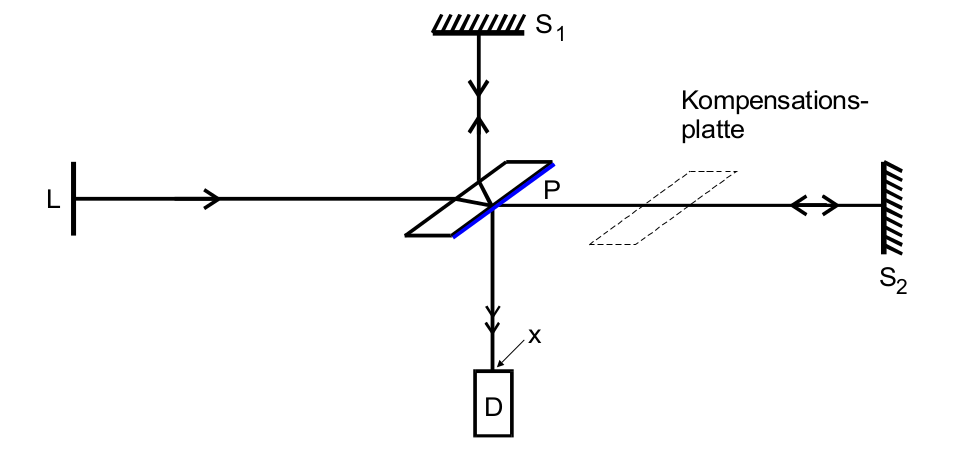
\includegraphics[height=5cm]{logos/SchemaInterf.png}
  \caption{Schematischer Aufbau des Michelson-Interferometers \cite{Anleitung}.}
  \label{fig:SA}
\end{figure}

Wird nun der Spiegel um $\Delta d$ verschoben so zählt der Detektor die autrettenden
Intensitätsmaxima. Daraus kann dann mit der Formel \cite{Anleitung}
\begin {equation}
  \Delta d = z \cdot \frac{\lambda}{2}
  \label{eqn:dd}
\end{equation}
die Wellenlänge $\lambda$ brechnet werden, dabei bezweichnet $z$ die Anzahl der
Interferenzmaxima. \\
Ist nun die Wellenlänge bekannt und der Lichtstrahl durch läuft ein Weg mit der
Länge $b$ durch ein Medium mit einem zusätzlichen Brechungsindex $ n + \Delta n$,
dann verändert sich auch der Wegunterschied der beiden interferierenden Strahlen.
Dieser beträgt nun genau $\Delta n \cdot b$. Diesen Wegunterschied wird nun
vergrößert in dem der Gasdruck in der Messzelle die die Strahlen passieren erhöht
wird (siehe Darstellung \ref{fig:KA}). Nun folgt für den Wegunterschied
\begin{equation}
  b \cdot \Delta n = z \frac{\lambda}{2}\;.
  \label{eqn:n}
\end{equation}
So kann nun der Brechungsindex $\Delta n$ bestimmt werden.
